%===============================================================================%
\chapter{Applications and Visualisations} \label{chapter:application}
%===============================================================================%

%300 words on how the data can be used.
\lipsum[1-2]

%-------------------------------------------------------------------------------%
\section{Footfall Landscape of United Kingdom}
%-------------------------------------------------------------------------------%
% how the data can be used in understanding the nature of the places they are installed. Aggregated to different level.
\lipsum[3]
\subsection{UK footfall index}
% Combining them together to have and index UK. How footfall has gone up or down every week compared to last week or compared to last year.
\lipsum[1]

\begin{figure*}
  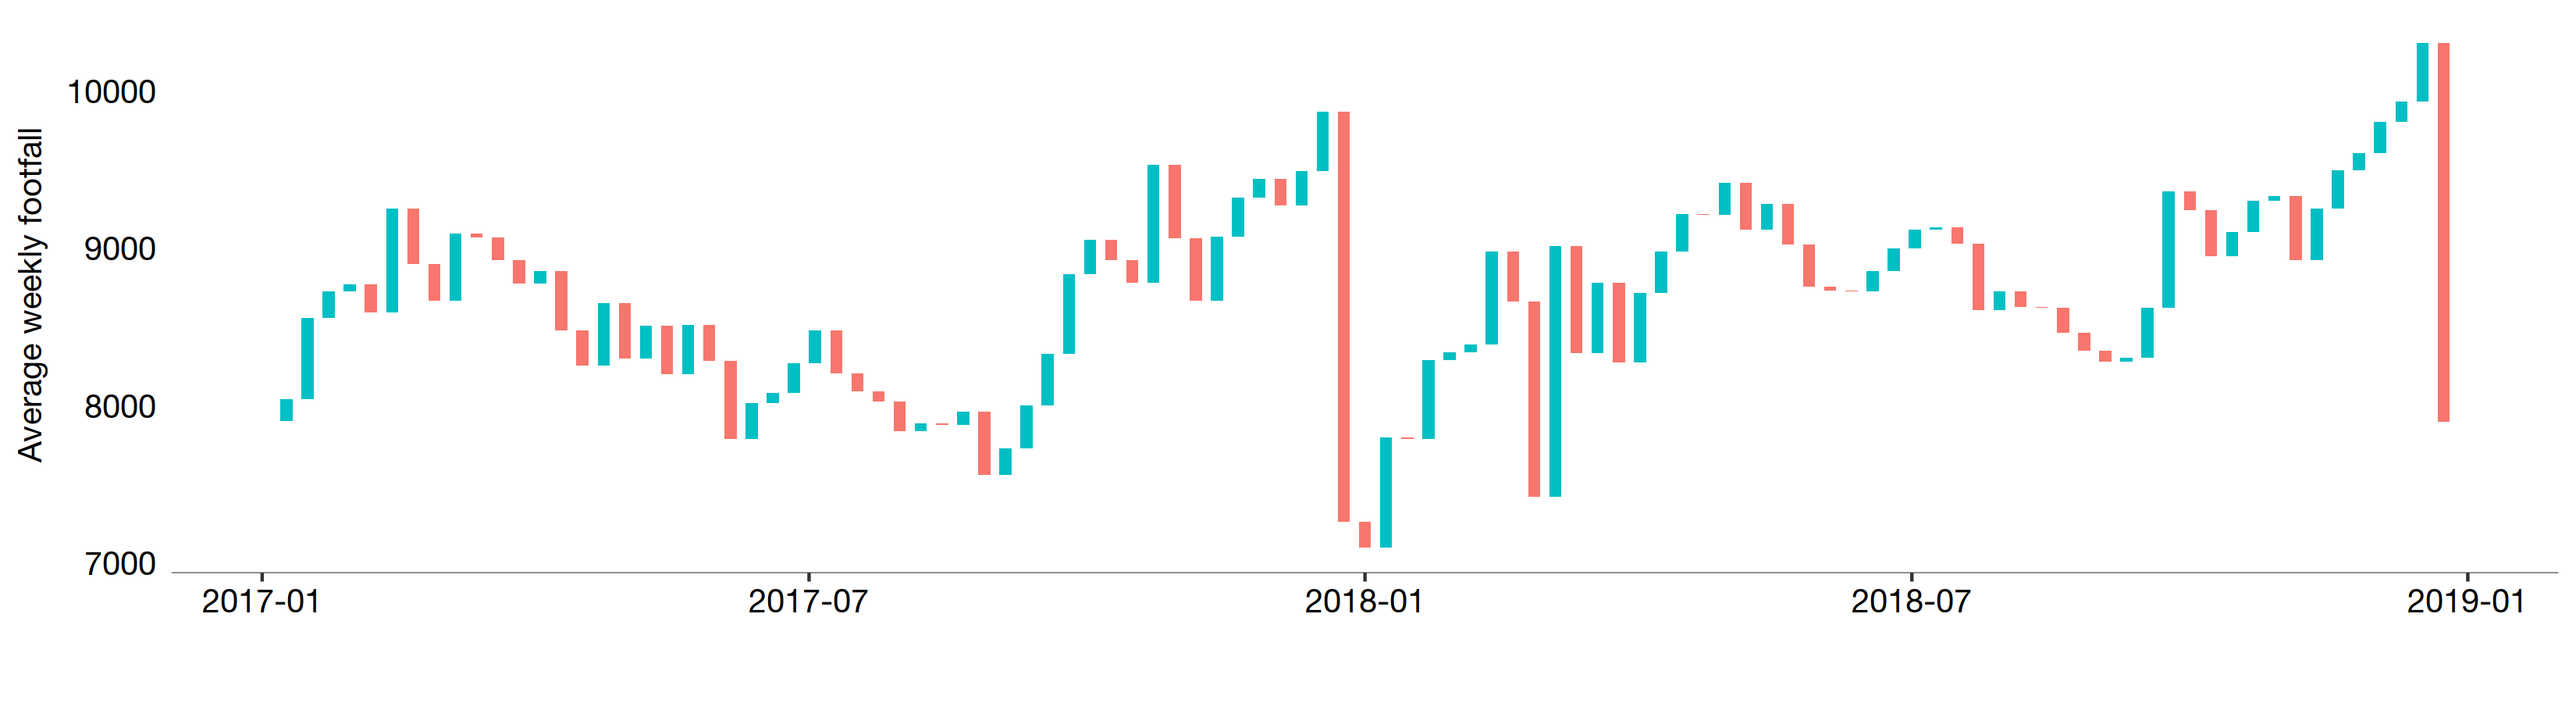
\includegraphics[trim={0 25 0 10},clip]{images/applications-footfall-index.png}
  \caption{}
  \label{}
\end{figure*}

\subsection{City wise indices}
% The footfall profiles in a day can be used to see how different cities work differently.
\lipsum[1-2]

\begin{figure*}
  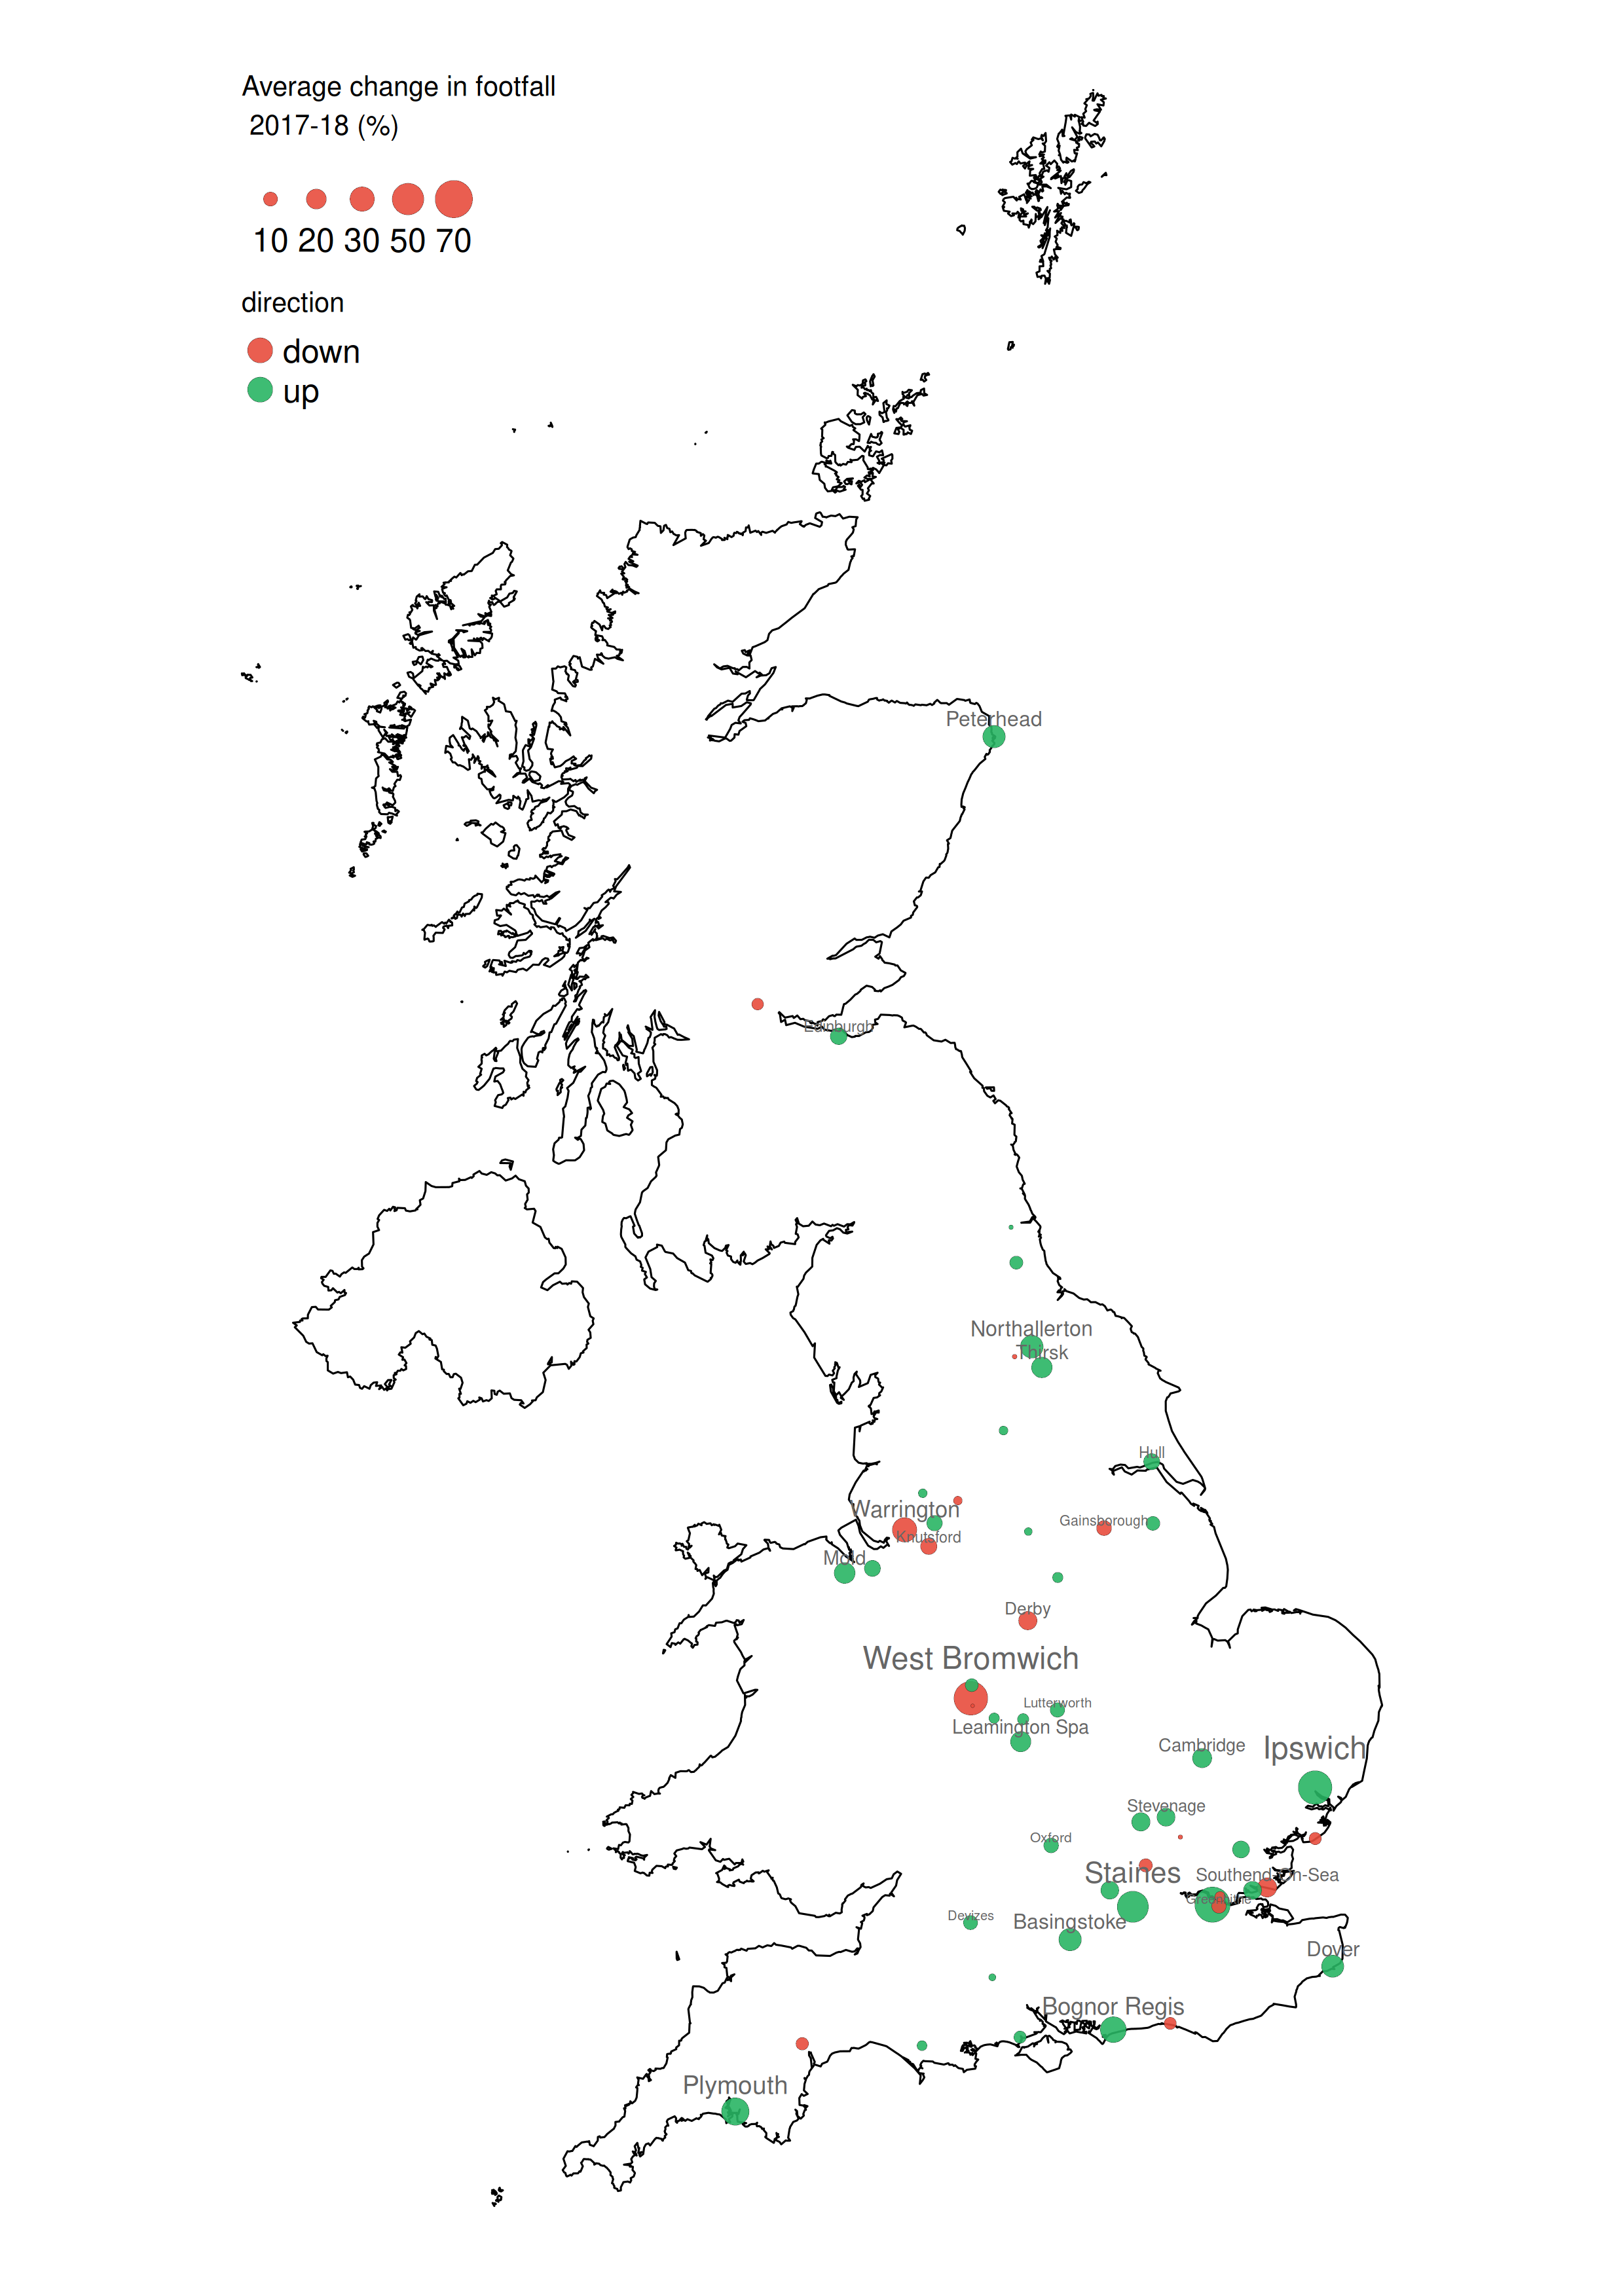
\includegraphics[trim={0 0 0 0},clip]{images/applications-cities-rank.png}
  \caption{}
  \label{}
\end{figure*}

\lipsum[1]

\begin{figure*}
  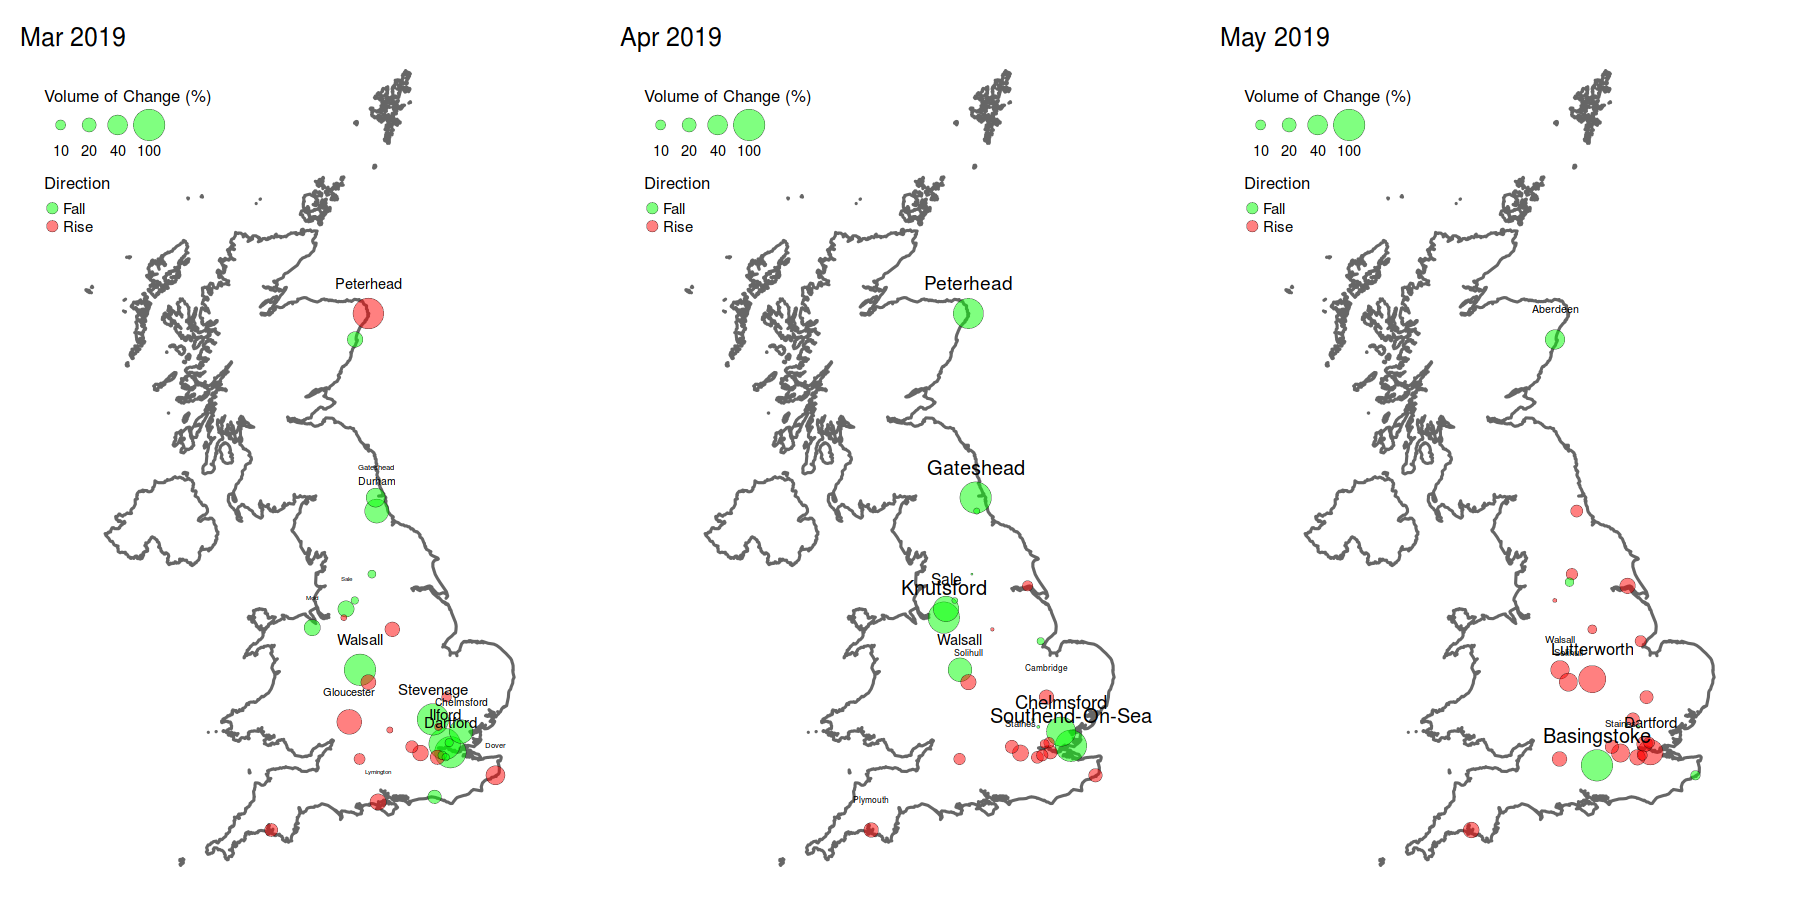
\includegraphics[trim={0 12 0 0},clip]{images/applications-city-indices.png}
  \caption{The profiles can be tracked longitudinally to reveal nature and change}
  \label{}
\end{figure*}

\lipsum[1]

\begin{figure*}
  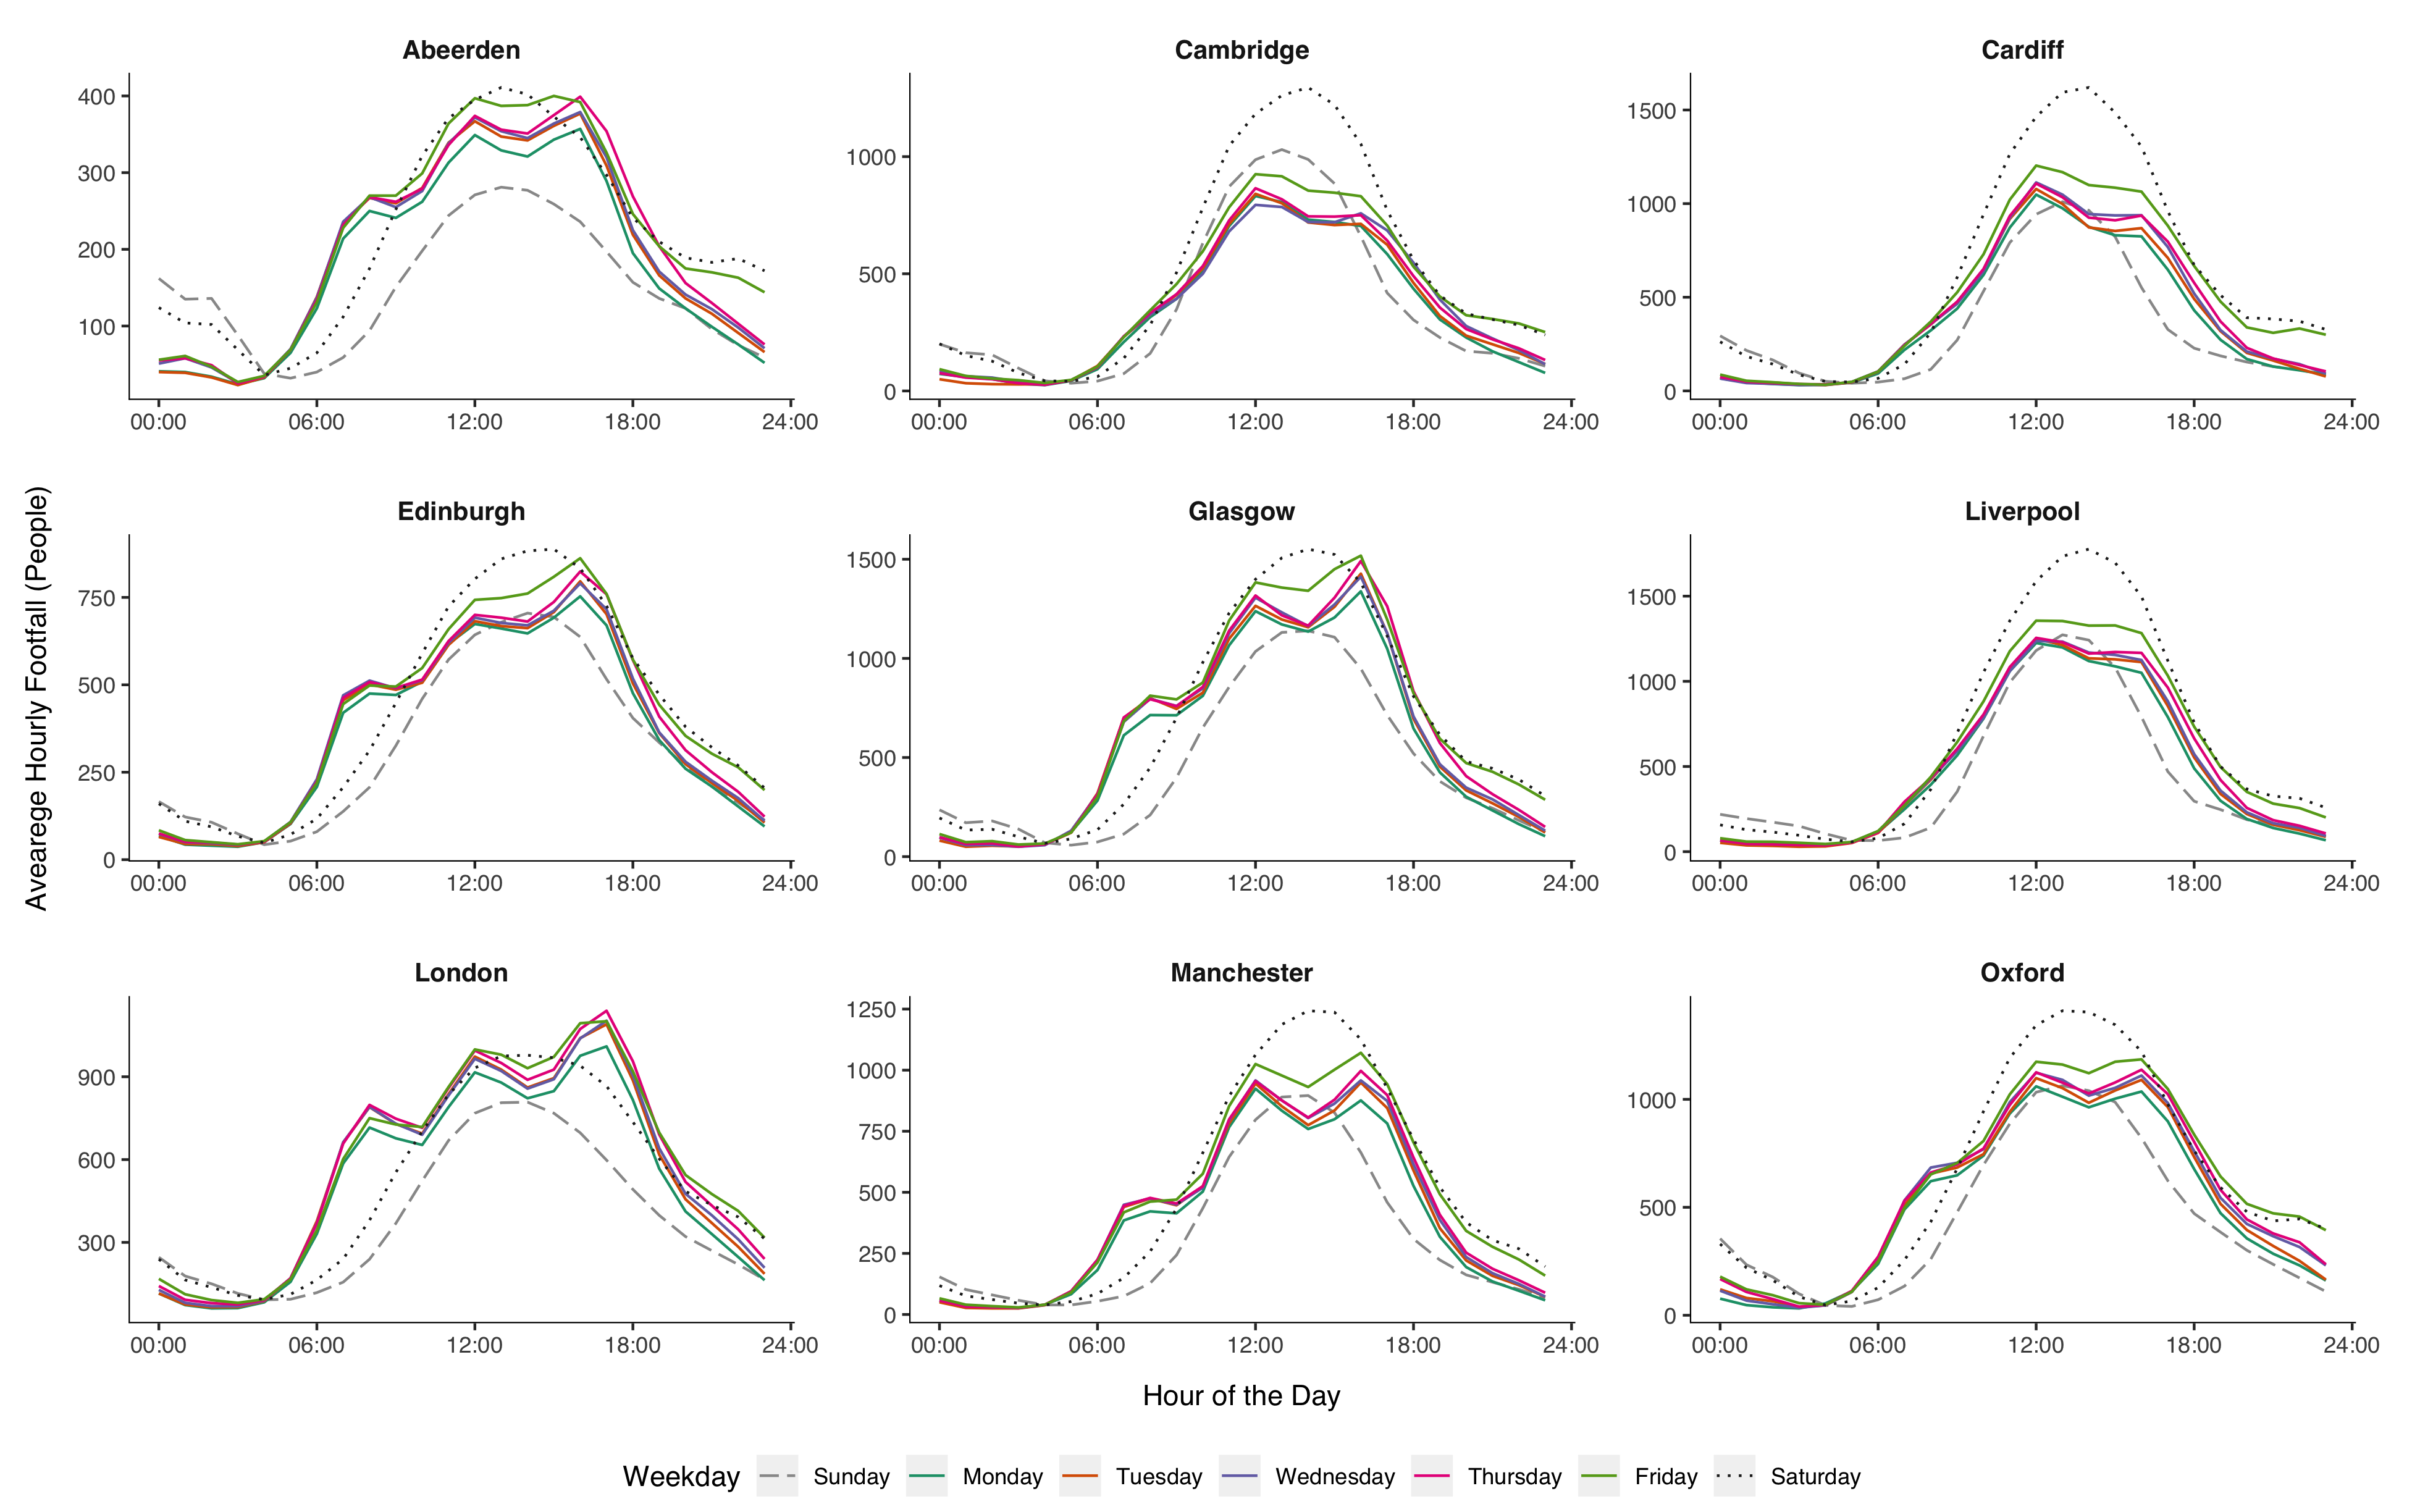
\includegraphics[trim={0 10 0 0},clip]{images/applications-city-profiles.png}
  \caption{The profiles can be tracked longitudinally to reveal nature and change}
  \label{}
\end{figure*}

\lipsum[1]

\subsection{Location comparisons}
% the locations can vary widely and their profiles can show their nature. compare couple of locations to show difference in character.
\lipsum[1]

\begin{figure*}
  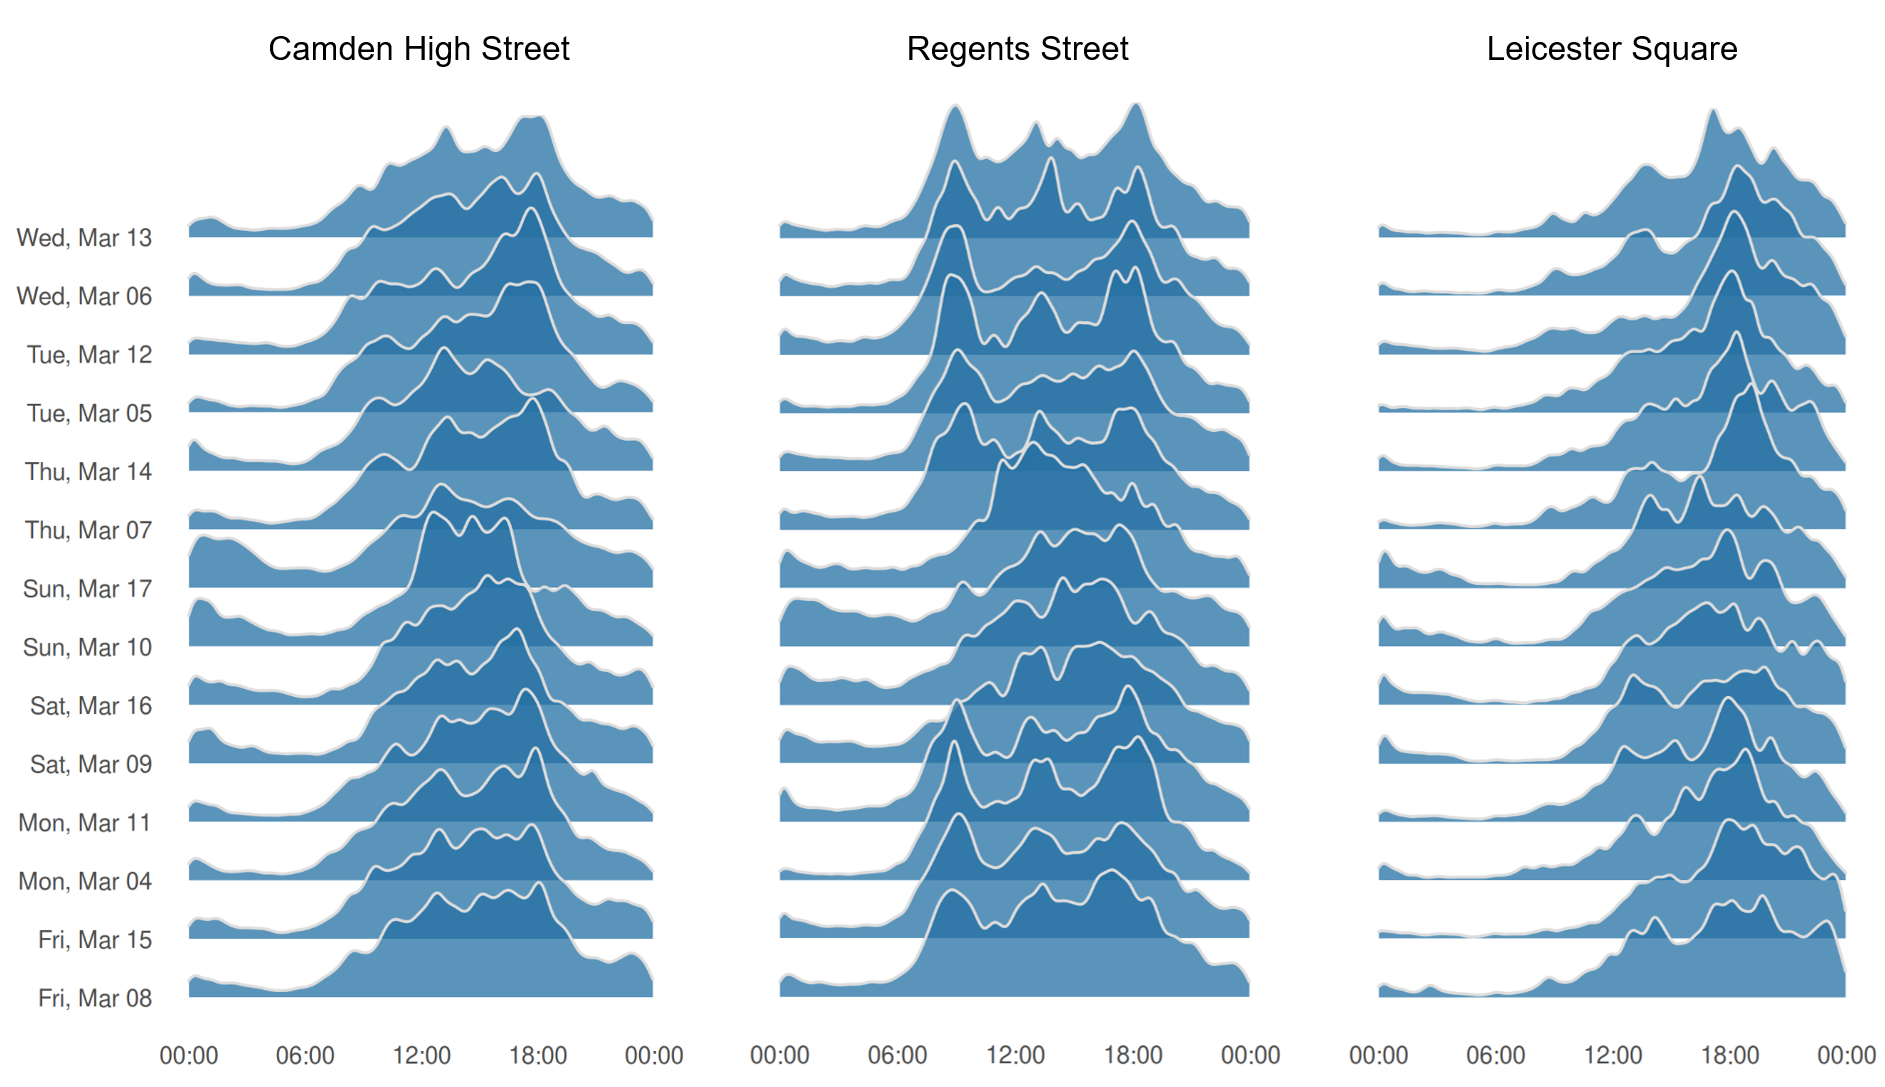
\includegraphics[trim={0 10 0 0},clip]{images/applications-location-profiles.png}
  \caption{The profiles can be tracked longitudinally to reveal nature and change}
  \label{}
\end{figure*}

\subsection{Longitudinal analysis}
% The profiles can be tracked longitudinally to reveal nature and change of nature over time. Footfall calendar

\lipsum[1]

\lipsum[1-2]

\cleartoleftpage
\newgeometry{
  left=20mm,
  textwidth=122mm,
  marginparsep=7mm,
  marginparwidth=43mm
}
\begin{figure*}
  \forceversofloat
  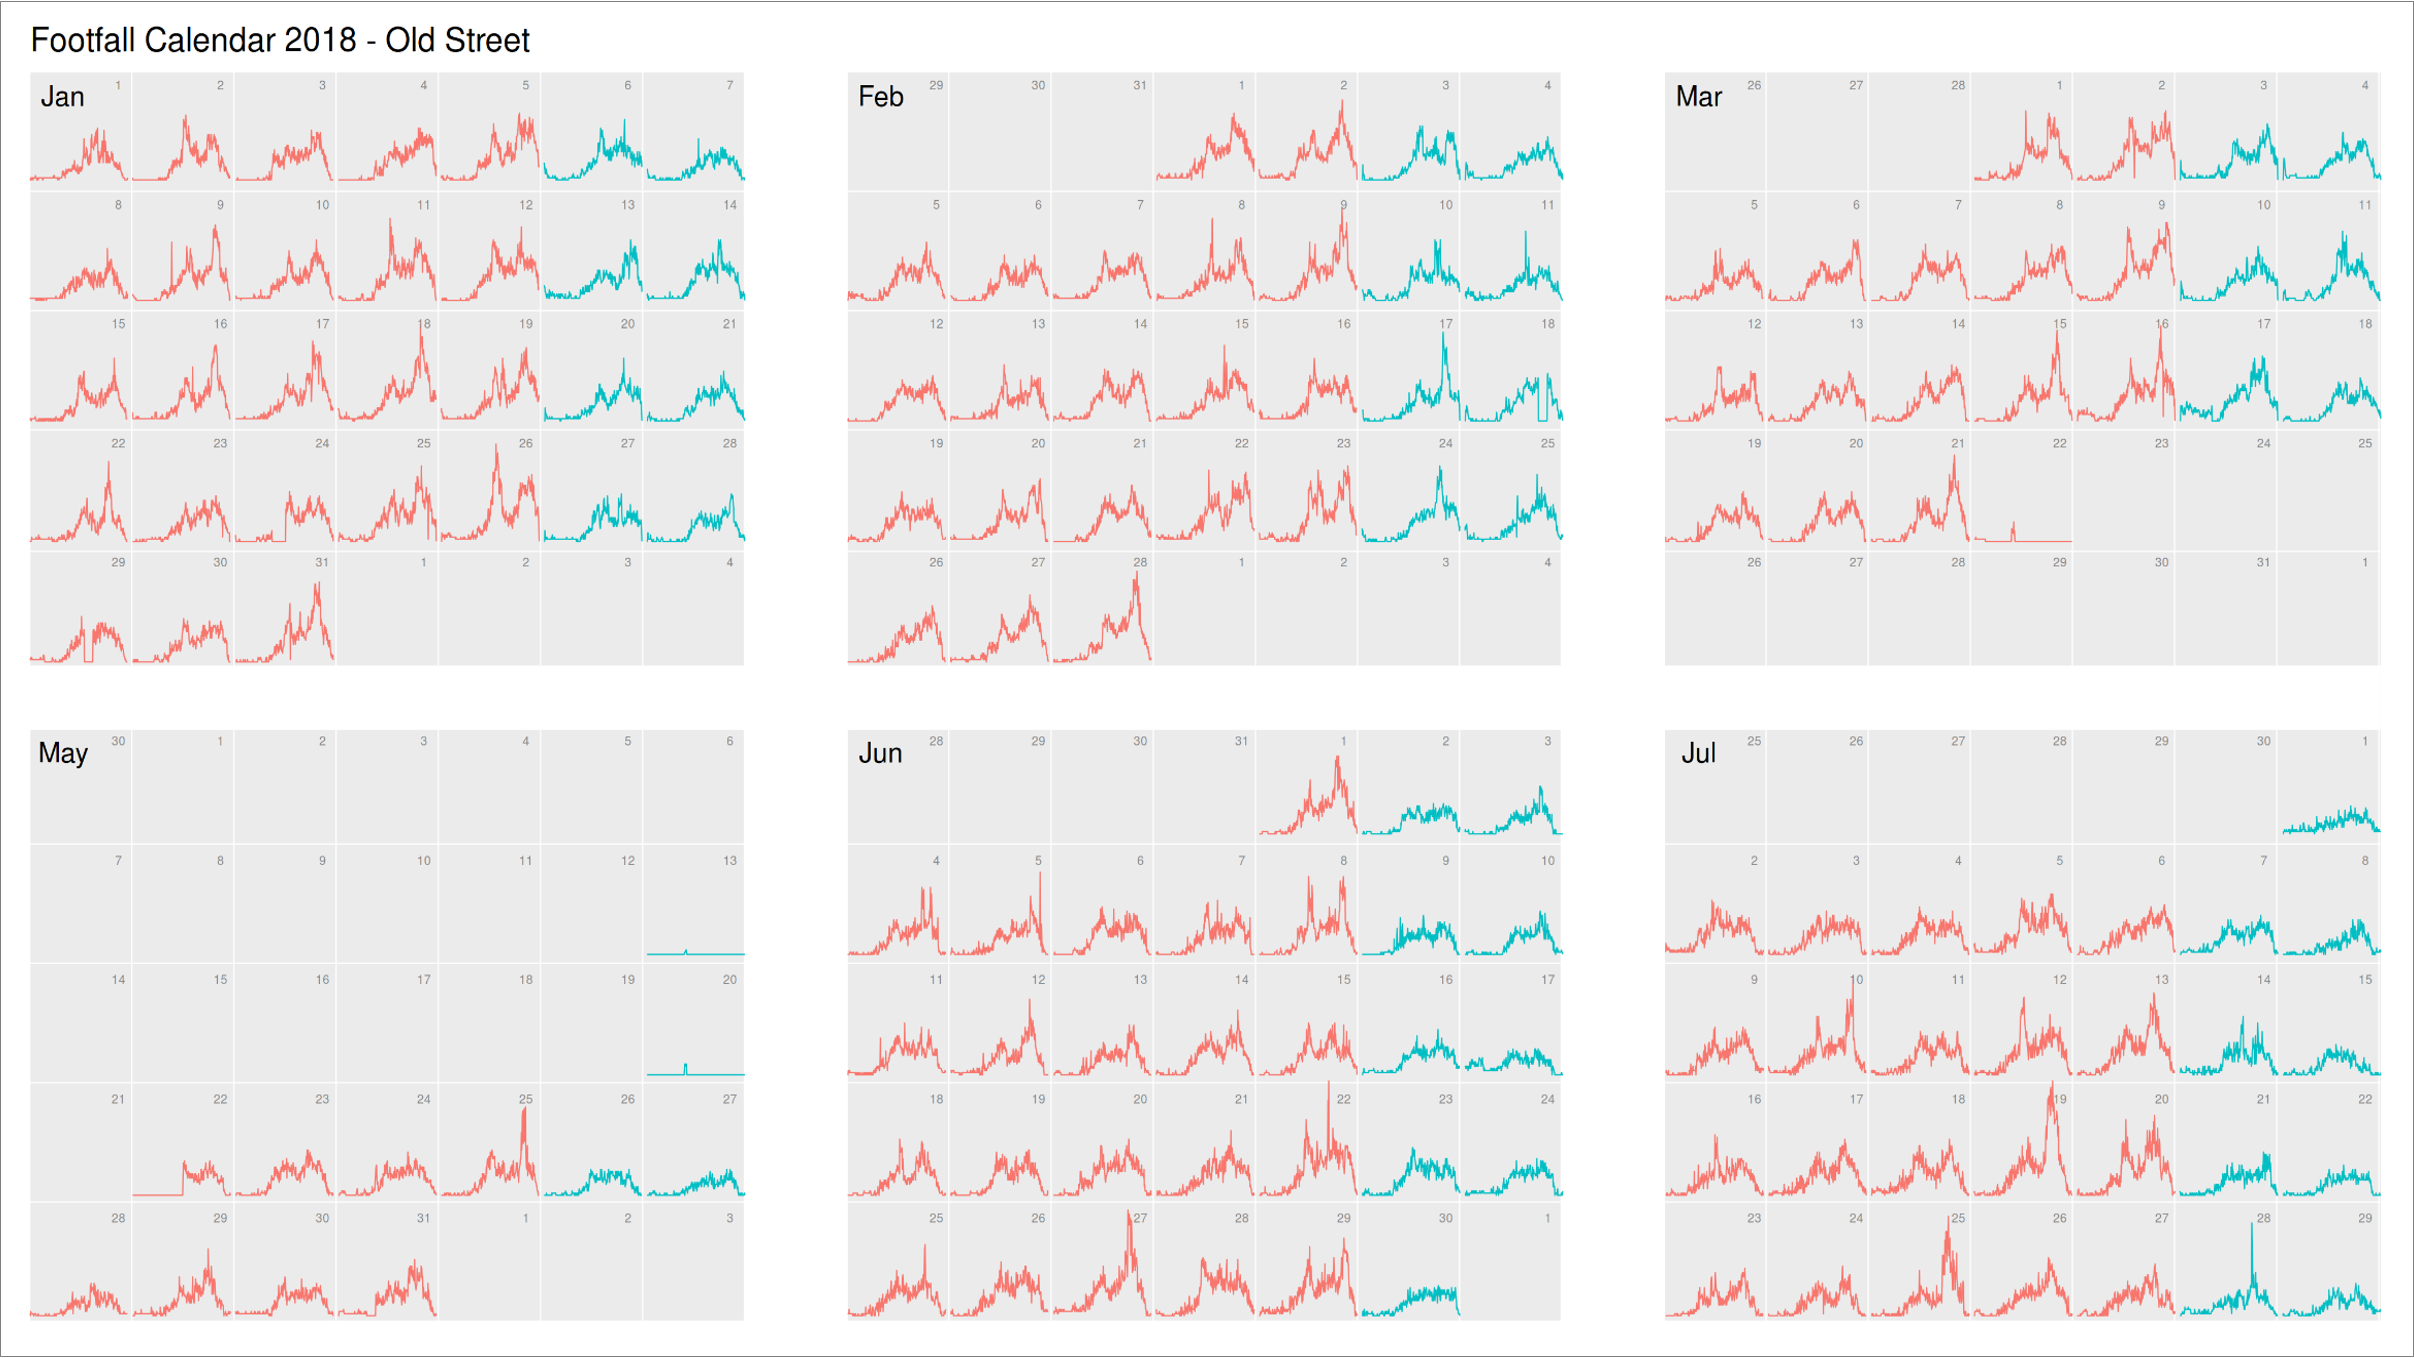
\includegraphics[width=172mm,trim={0 0 1310 -42},clip]{images/applications-footfall-calendar.png}
  \caption{Footfall calendar showing the profiles of daily volume of footfall at Old Street, London.}
  \label{}
\end{figure*}
\clearpage
\begin{figure*}
  \forcerectofloat
  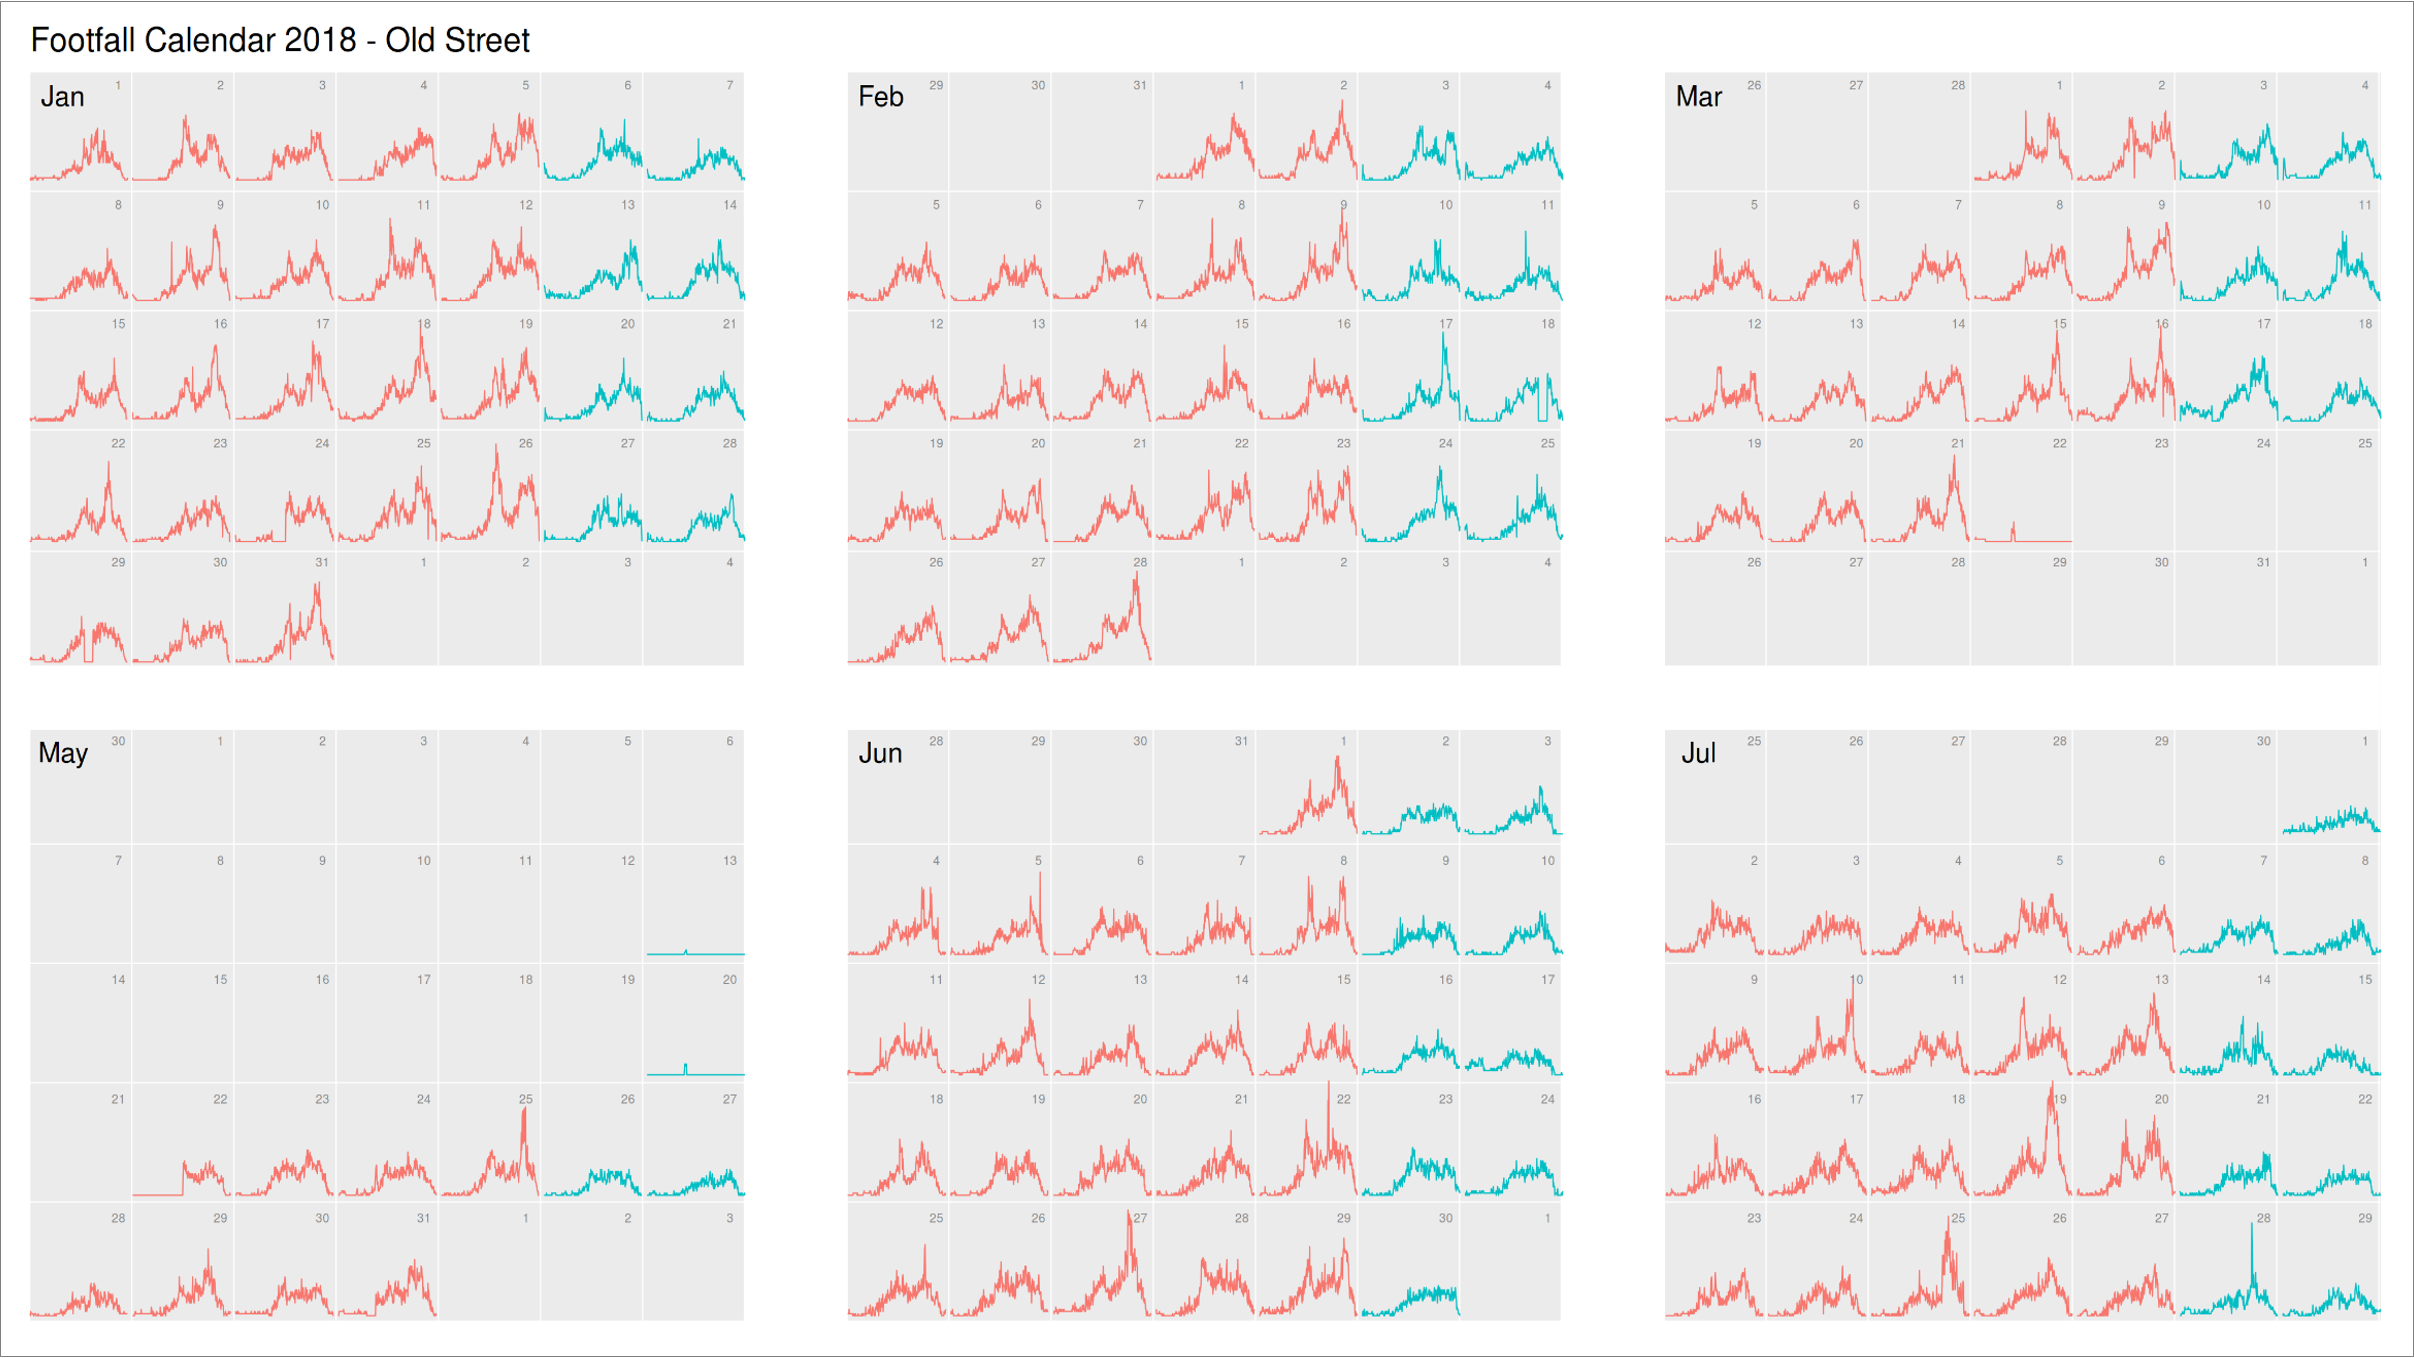
\includegraphics[width=172mm,trim={1315 0 0 0},clip]{images/applications-footfall-calendar.png}
  \caption[]{}
  \label{}
\end{figure*}
\restoregeometry
\clearpage


%-------------------------------------------------------------------------------%
\section{Event Detection}
%-------------------------------------------------------------------------------%

\lipsum[1]

% how the data is longitudinal and can be used to detect events from the changes in footfall.

% Discuss the events

\begin{figure*}
  \forceversofloat
  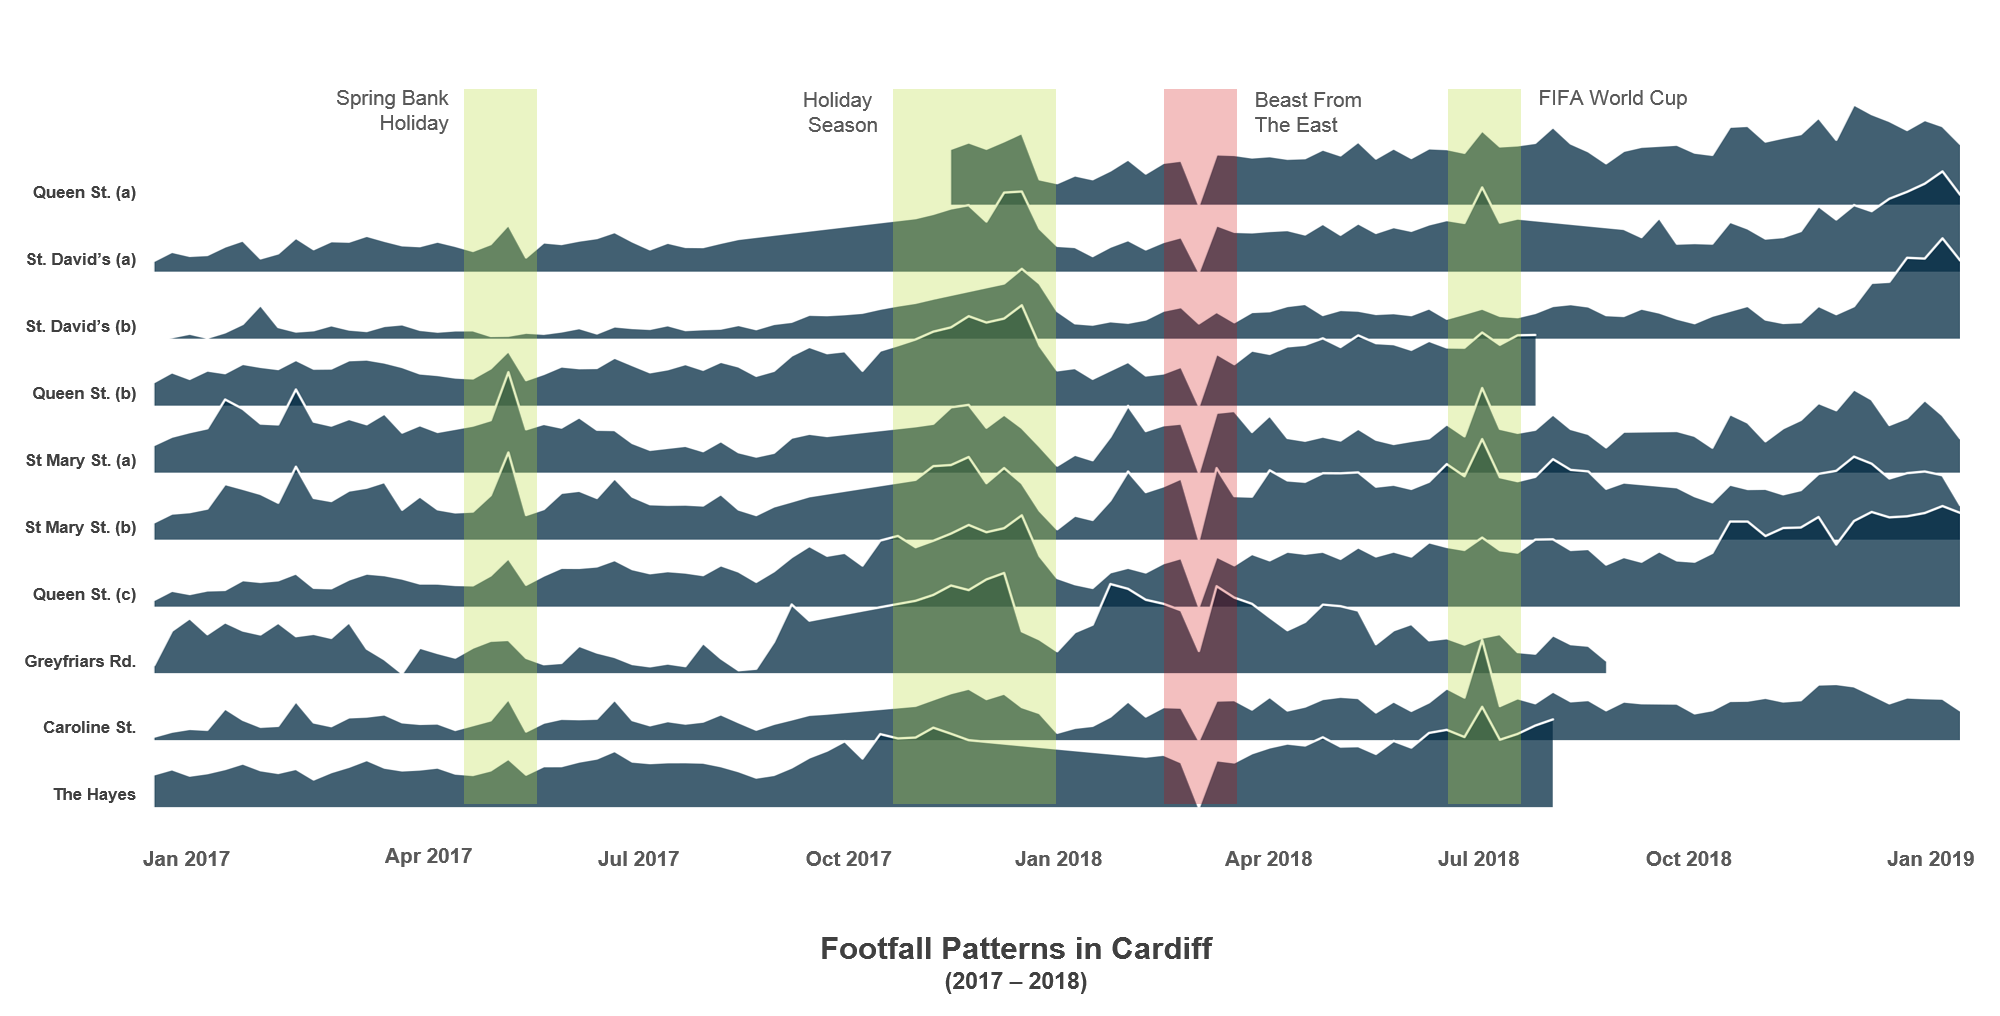
\includegraphics[trim={0 50 0 0},clip]{images/applications-cardiff-footfall.png}
  \caption{}
  \label{}
\end{figure*}

\subsection{Football world cup}
% micro site variations could be identified as well.

% match day compared to other days.
% post match celebrations graphic.

%-------------------------------------------------------------------------------%
\section{Pedestrian Flows}
%-------------------------------------------------------------------------------%
Detecting general trends in flow of people between spatial locations is neither obvious nor an easy task due the high cost of capturing these movements without compromising the privacy of those involved. This research intends to address this problem by examining the movement of people in a SmartStreetSensors network at a fine spatial and temporal resolution. A novel methodology to the field of Big Data using mathematical models from information theory is introduced, taking an area in central London as a case study.

\begin{figure*}
  \forceversofloat
  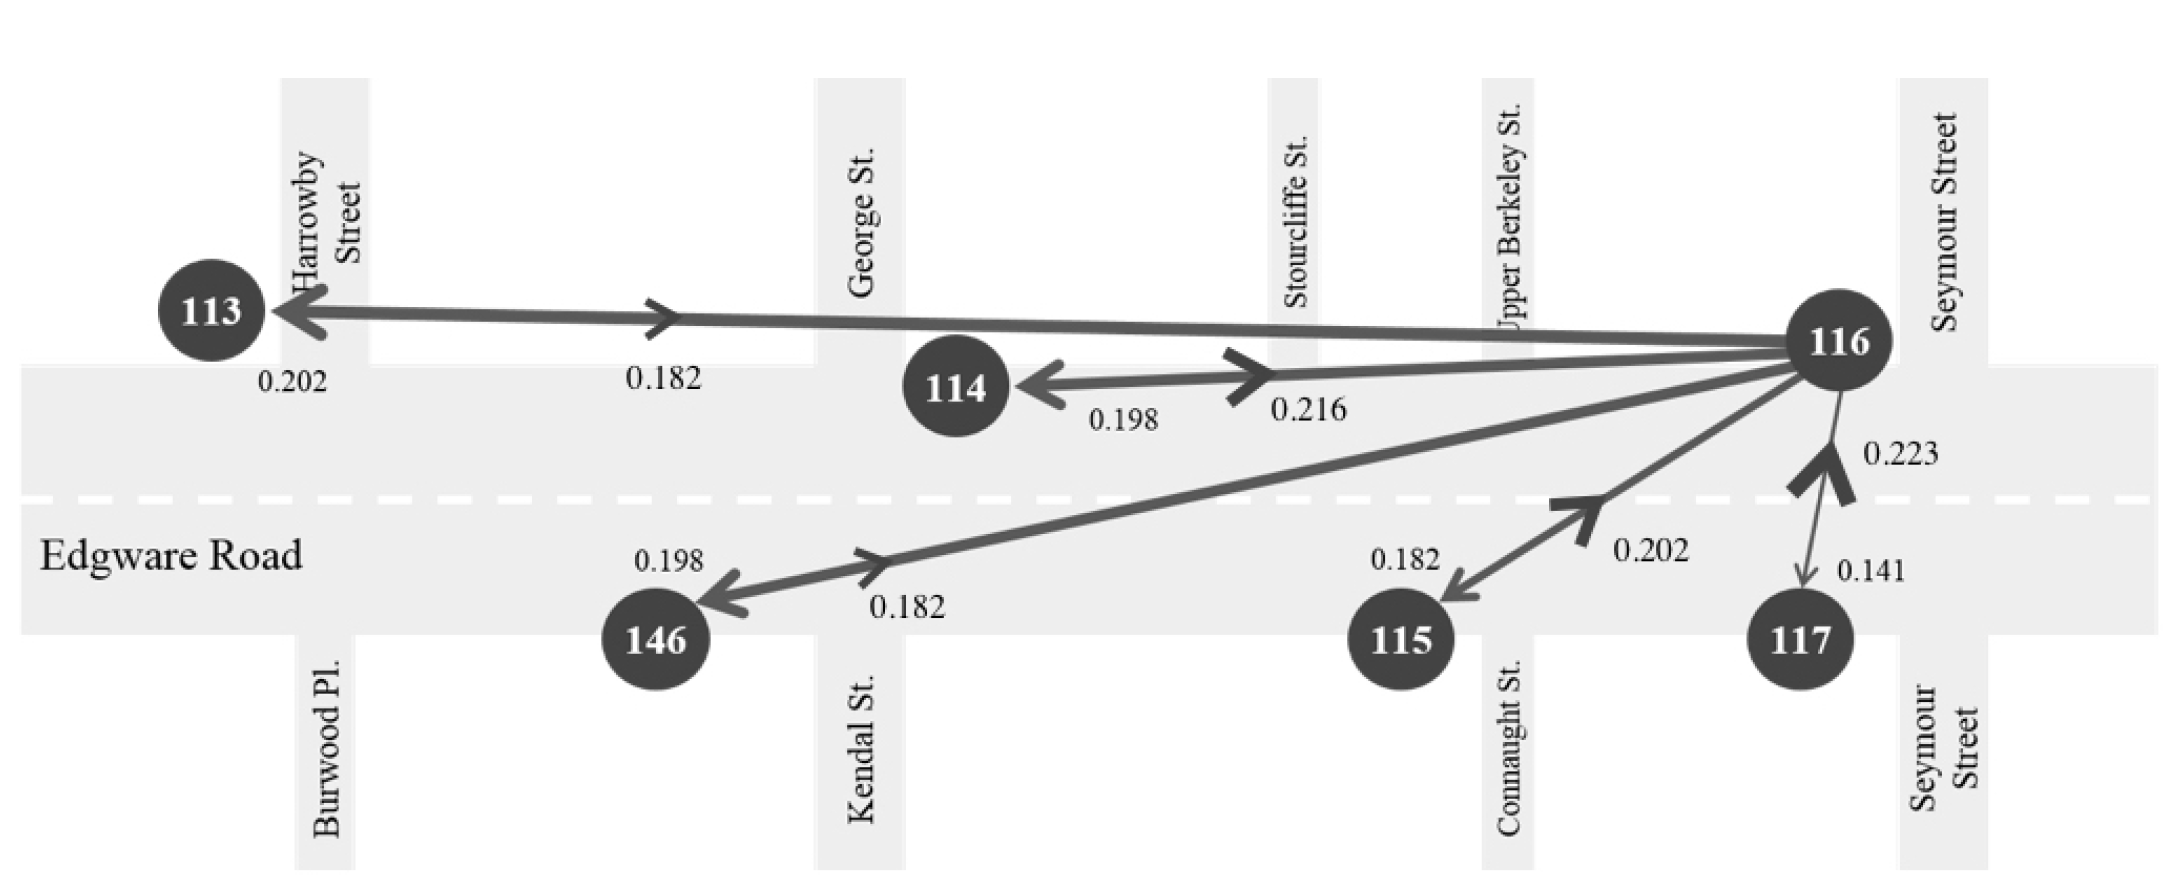
\includegraphics[trim={0 0 0 0},clip]{images/applications-transfer-entropy.png}
  \caption{}
  \label{}
\end{figure*}

Consider the array of sensors shown at Figure 2. Let’s assume that we have a flow of people walking past the location 116 and then diffusing towards the remaining sensors. Counts generated by the sensor are aggregated per five minute intervals, so if, for example, it takes one minute to walk from the location 116 to the location 117, the number of people detected at 117 from minutes 2 to 5, would correspond to the percentage of people detected at 116 from minutes 1 to 4. In other words, the similarity between the time series of counts at the locations under consideration are correlated. The aim is to, without actually tracking people, provide a measure for the size of the flow between each pair of sensors.  One way to accomplish this, is to think of this motion of people as flows of information among distinctive sources, so we can relate the number of people reaching one sensor from another by measuring the uncertainty between two interacting random variables. For this, we used an information theory concept known as Transfer Entropy TE defined by:

where t indicates a given point in time. eq 1 measures the reduction in uncertainty at yt, given xt and yt-1. In comparison with the case when only yt-1 is known.
If this measure is applied directly to our people's movement problem and X = location i, Y = location j and t runs for a whole day, the TE would represent an idicator fo the direction of the flow, as the counts at yt+1 are more accurately estimated using the ifnormation of xt.


Taking again Figure 2 as a reference, we measured the TE between sensor 116 and the rest of the sensors. The walking time is not constant and each sensor has counts at all times i, i.e., there are people passing by these sensors that came from locations outside the network. The numbers at each line represent the TE measured between each pair of sensor locations. The largest TE value found was between 117 to 115. The asymmetry of the TE is clear here, as the value in the opposite direction (115 to 117) is considerably lower. Another interesting value is the pair 116-117, where TE(116,117) << TE(117,116). This demonstrates that in this four-way crossing the predominant direction of flow is from location 117 to location 116 (from the bottom of the figure upwards, or from west to east in reality). These results suggest that, in general there is a larger flow of people from West side to East side of Edgware road and larger flow of people from South to North. The results are consistent with our intuition that there is a larger flow of people from South to North along this road towards the Edgware road underground station.  
There is still a series of situations yet to be addressed by this model, such as the decay of probabilities with distance and the number of interventions of opportunity encountered by people while walking from one sensor to another. However, this first initial set of results is encouraging.  

% Another approach for interpolation is Geo-propagation
% It can be promising as well.

%-------------------------------------------------------------------------------%
\section{Discussion}
%-------------------------------------------------------------------------------%

% 500 words on what all the above does and how it can be taken forward.
% emphasize on other work that have been done based off this data

